%%%%%%%%%%%%%%%%%%%%%%%%%%%%%%%%%%%%%%%%%%%%%%
%% Compile: XeLaTeX BibTeX XeLaTeX XeLaTeX
%% Handout: Antonio Machicao y Priemer
%% Course: GK Linguistik
%%%%%%%%%%%%%%%%%%%%%%%%%%%%%%%%%%%%%%%%%%%%%%

%\documentclass[a4paper,10pt, bibtotoc]{beamer}
\documentclass[10pt,handout]{beamer}

%%%%%%%%%%%%%%%%%%%%%%%%
%%     PACKAGES      
%%%%%%%%%%%%%%%%%%%%%%%%

%%%%%%%%%%%%%%%%%%%%%%%%
%%     PACKAGES       %%
%%%%%%%%%%%%%%%%%%%%%%%%



%\usepackage[utf8]{inputenc}
%\usepackage[vietnamese, english,ngerman]{babel}   % seems incompatible with german.sty
%\usepackage[T3,T1]{fontenc} breaks xelatex
\usepackage{lmodern}

\usepackage{amsmath}
\usepackage{amsfonts}
\usepackage{amssymb}
%% MnSymbol: Mathematische Klammern und Symbole (Inkompatibel mit ams-Packages!)
%% Bedeutungs- und Graphemklammern: $\lsem$ Tisch $\rsem$ $\langle TEXT \rangle$ $\llangle$ TEXT $\rrangle$ 
\usepackage{MnSymbol}
%% ulem: Strike out
\usepackage[normalem]{ulem}  

%% Special Spaces (s. Commands)
\usepackage{xspace}				
\usepackage{setspace}
%	\onehalfspacing

%% mdwlist: Special lists
\usepackage{mdwlist}	

\usepackage[noenc,safe]{tipa}

% maybe define \textipa to use \originalTeX to avoid problems with `"'.
%
%	\ex \textipa{\originalTeX [pa.pa."g\t{aI}]}

%

\usepackage{etex}		%For Forest bug

%
%\usepackage{jambox}
%


%\usepackage{forest-v105}
%\usepackage{modified-langsci-forest-setup}

\usepackage{xeCJK}
\setCJKmainfont{SimSun}


%\usepackage{natbib}
%\setcitestyle{notesep={:~}}




% for toggles
\usepackage{etex}



% Fraktur!
\usepackage{yfonts}

\usepackage{url}

% für UDOP
\usepackage{adjustbox}


%% huberlin: Style sheet
%\usepackage{huberlin}
\usepackage{hu-beamer-includes-pdflatex}
\huberlinlogon{0.86cm}


%% Last Packages
%\usepackage{hyperref}	%URLs
%\usepackage{gb4e}		%Linguistic examples

% sorry this was incompatible with gb4e and had to go.
%\usepackage{linguex-cgloss}	%Linguistic examples (patched version that works with jambox

\usepackage{multirow}  %Mehrere Zeilen in einer Tabelle
%\usepackage{array}
\usepackage{marginnote}	%Notizen




%%%%%%%%%%%%%%%%%%%%%%%%%%%%%%%%%%%%%%%%%%%%%%%%%%%%
%%%             Preamble's End                   
%%%%%%%%%%%%%%%%%%%%%%%%%%%%%%%%%%%%%%%%%%%%%%%%%%%% 

\begin{document}
	
	%%%%%%%%%%%%%%%%%%%%%%%%%%%%%%%%%%%%%%%%%%%%%%%%%%%%
%%%          Commands                            %%%
%%%%%%%%%%%%%%%%%%%%%%%%%%%%%%%%%%%%%%%%%%%%%%%%%%%%

%%%%%%%%%%%%%%%%%%%%%%%%%%%%%%%%
% German quotation marks:
\newcommand{\gqq}[1]{\glqq{}#1\grqq{}}		%double
\newcommand{\gq}[1]{\glq{}#1\grq{}}			%simple


%%%%%%%%%%%%%%%%%%%%%%%%%%%%%%%%
% Abbreviations in German
% package needed: xspace
% Short space in German abbreviations: \,	
\newcommand{\idR}{\mbox{i.\,d.\,R.}\xspace}
\newcommand{\su}{\mbox{s.\,u.}\xspace}
%\newcommand{\ua}{\mbox{u.\,a.}\xspace}       % in abbrev
%\newcommand{\zB}{\mbox{z.\,B.}\xspace}       % in abbrev
%\newcommand{\s}{s.~}
%not possibel: \dh --> d.\,h.


%%%%%%%%%%%%%%%%%%%%%%%%%%%%%%%%
%Abbreviations in English
\newcommand{\ao}{a.o.\ }	% among others
\newcommand{\cf}[1]{(cf.~#1)}	% confer = compare
\renewcommand{\ia}{i.a.}	% inter alia = among others
\newcommand{\ie}{i.e.~}	% id est = that is
\newcommand{\fe}{e.g.~}	% exempli gratia = for example
%not possible: \eg --> e.g.~
\newcommand{\vs}{vs.\ }	% versus
\newcommand{\wrt}{w.r.t.\ }	% with respect to


%%%%%%%%%%%%%%%%%%%%%%%%%%%%%%%%
% Dash:
\newcommand{\gs}[1]{--\,#1\,--}


%%%%%%%%%%%%%%%%%%%%%%%%%%%%%%%%
% Rightarrow with and without space
\def\ra{\ensuremath\rightarrow}			%without space
\def\ras{\ensuremath\rightarrow\ }		%with space


%%%%%%%%%%%%%%%%%%%%%%%%%%%%%%%%
%% X-bar notation

%% Notation with primes (not emphasized): \xbar{X}
\newcommand{\MyPxbar}[1]{#1$^{\prime}$}
\newcommand{\xxbar}[1]{#1$^{\prime\prime}$}
\newcommand{\xxxbar}[1]{#1$^{\prime\prime\prime}$}

%% Notation with primes (emphasized): \exbar{X}
\newcommand{\exbar}[1]{\emph{#1}$^{\prime}$}
\newcommand{\exxbar}[1]{\emph{#1}$^{\prime\prime}$}
\newcommand{\exxxbar}[1]{\emph{#1}$^{\prime\prime\prime}$}

% Notation with zero and max (not emphasized): \xbar{X}
\newcommand{\zerobar}[1]{#1$^{0}$}
\newcommand{\maxbar}[1]{#1$^{\textsc{max}}$}

% Notation with zero and max (emphasized): \xbar{X}
\newcommand{\ezerobar}[1]{\emph{#1}$^{0}$}
\newcommand{\emaxbar}[1]{\emph{#1}$^{\textsc{max}}$}

%% Notation with bars (already implemented in gb4e):
% \obar{X}, \ibar{X}, \iibar{X}, \mbar{X} %Problems with \mbar!
%
%% Without gb4e:
\newcommand{\overbar}[1]{\mkern 1.5mu\overline{\mkern-1.5mu#1\mkern-1.5mu}\mkern 1.5mu}
%
%% OR:
\newcommand{\MyPibar}[1]{$\overline{\textrm{#1}}$}
\newcommand{\MyPiibar}[1]{$\overline{\overline{\textrm{#1}}}$}
%% (emphasized):
\newcommand{\eibar}[1]{$\overline{#1}$}
\newcommand{\eiibar}[1]{\overline{$\overline{#1}}$}

%%%%%%%%%%%%%%%%%%%%%%%%%%%%%%%%
%% Subscript & Superscript: no italics
\newcommand{\MyPdown}[1]{$_{\textrm{#1}}$}
\newcommand{\MyPup}[1]{$^{\textrm{#1}}$}


%%%%%%%%%%%%%%%%%%%%%%%%%%%%%%%%
% Objekt language marking:
%\newcommand{\obj}[1]{\glqq{}#1\grqq{}}	%German double quotes
%\newcommand{\obj}[1]{``#1''}			%English double quotes
\newcommand{\MyPobj}[1]{\emph{#1}}		%Emphasising


%%%%%%%%%%%%%%%%%%%%%%%%%%%%%%%%
%% Semantic types (<e,t>), features, variables and graphemes in angled brackets 

%%% types and variables, in math mode: angled brackets + italics + no space
%\newcommand{\type}[1]{$<#1>$}

%%% OR more correctly: 
%%% types and variables, in math mode: chevrons! + italics + no space
\newcommand{\MyPtype}[1]{$\langle #1 \rangle$}

%%% features and graphemes, in math mode: chevrons! + italics + no space
\newcommand{\abe}[1]{$\langle #1 \rangle$}


%%% features and graphemes, in math mode: chevrons! + no italics + space
\newcommand{\ab}[1]{$\langle$#1$\rangle$}  %%same as \abu  
\newcommand{\abu}[1]{$\langle$#1$\rangle$} %%Umlaute

%%% Notizen
\renewcommand{\marginfont}{\singlespacing}
\renewcommand{\marginfont}{\footnotesize}
\renewcommand{\marginfont}{\color{black}}

\newcommand{\myp}[1]{%
	\marginnote{%
		\begin{spacing}{1}
			\vspace{-\baselineskip}%
			\color{red}\footnotesize#1
		\end{spacing}
	}
}
%%%%%%%%%%%%%%%%%%%%%%%%%%%%%%%%
%% Outputbox
\newcommand{\outputbox}[1]{\noindent\fbox{\parbox[t][][t]{0.98\linewidth}{#1}}\vspace{0.5em}}

%%%%%%%%%%%%%%%%%%%%%%%%%%%%%%%%
%% (Syntactic) Trees
% package needed: forest
%
%% Setting for simple trees
\forestset{
	MyP edges/.style={for tree={parent anchor=south, child anchor=north}}
}

%% this is taken from langsci-setup file
%% Setting for complex trees
%% \forestset{
%% 	sn edges/.style={for tree={parent anchor=south, child anchor=north,align=center}}, 
%% background tree/.style={for tree={text opacity=0.2,draw opacity=0.2,edge={draw opacity=0.2}}}
%% }

\newcommand\HideWd[1]{%
	\makebox[0pt]{#1}%
}


%%%%%%%%%%%%%%%%%%%%%%%%%%%%%%%%%%%%%%%%%%%%%%%%%%%%
%%%          Useful commands                     %%%
%%%%%%%%%%%%%%%%%%%%%%%%%%%%%%%%%%%%%%%%%%%%%%%%%%%%

%%%%%%%%%%%%%%%%%%%%%
%% FOR ITEMS:
%\begin{itemize}
%  \item<2-> from point 2
%  \item<3-> from point 3 
%  \item<4-> from point 4 
%\end{itemize}
%
% or: \onslide<2->
% or: \pause

%%%%%%%%%%%%%%%%%%%%%
%% VERTICAL SPACE:
% \vspace{.5cm}
% \vfill

%%%%%%%%%%%%%%%%%%%%%
% RED MARKING OF TEXT:
%\alert{bis spätestens Mittwoch, 18 Uhr}

%%%%%%%%%%%%%%%%%%%%%
%% RESCALE BIG TABLES:
%\scalebox{0.8}{
%For Big Tables
%}

%%%%%%%%%%%%%%%%%%%%%
%% BLOCKS:
%\begin{alertblock}{Title}
%Text
%\end{alertblock}
%
%\begin{block}{Title}
%Text
%\end{block}
%
%\begin{exampleblock}{Title}
%Text
%\end{exampleblock}


\newtoggle{uebung}
\newtoggle{loesung}
\newtoggle{toc}

% The toc is not needed on Handouts. Safe trees.
\mode<handout>{
\togglefalse{toc}
}

\newtoggle{hpsgvorlesung}\togglefalse{hpsgvorlesung}
\newtoggle{syntaxvorlesungen}\togglefalse{syntaxvorlesungen}

%\includecomment{psgbegriffe}
%\excludecomment{konstituentenprobleme}
%\includecomment{konstituentenprobleme-hinweis}

\newtoggle{konstituentenprobleme}\togglefalse{konstituentenprobleme}
\newtoggle{konstituentenprobleme-hinweis}\toggletrue{konstituentenprobleme-hinweis}

%\includecomment{einfsprachwiss-include}
%\excludecomment{einfsprachwiss-exclude}
\newtoggle{einfsprachwiss-include}\toggletrue{einfsprachwiss-include}
\newtoggle{einfsprachwiss-exclude}\togglefalse{einfsprachwiss-exclude}

\newtoggle{psgbegriffe}\toggletrue{psgbegriffe}

\newtoggle{gb-intro}\togglefalse{gb-intro}

	
%%%% ue-loesung
%%%% true: Übung & Lösungen (slides) / false: nur Übung (handout)
\togglefalse{ue-loesung}

%%%% ha-loesung
%%%% true: Hausaufgabe & Lösungen (slides) / false: nur Hausaufgabe (handout)
\togglefalse{ha-loesung}

%%%% toc
%%%% true: TOC am Anfang von Slides / false: keine TOC am Anfang von Slides
\toggletrue{toc}

%%%% sectoc
%%%% true: TOC für Sections / false: keine TOC für Sections (StM handout)
\toggletrue{sectoc}

%%%% gliederung
%%%% true: Gliederung für Sections / false: keine Gliederung für Sections
%	\toggletrue{gliederung}

%%%%%%%%%%%%%%%%%%%%%%%%%%%%%%%%%%%%%%%%%%%%%%%%%%%%
%%%             Metadata                         %%%
%%%%%%%%%%%%%%%%%%%%%%%%%%%%%%%%%%%%%%%%%%%%%%%%%%%%      

\title{Grundkurs Linguistik}

\subtitle{Semantik II \& Pragmatik I}

\author[aMyP]{
	{\small Antonio Machicao y Priemer}
%	\\
%	{\footnotesize \url{http://www.linguistik.hu-berlin.de/staff/amyp}\\
%	\href{mailto:mapriema@hu-berlin.de}{mapriema@hu-berlin.de}}
}

\institute{Institut für deutsche Sprache und Linguistik}

%%%%%%%%%%%%%%%%%%%%%%%%%      
\date{ }
%\publishers{\textbf{6. linguistischer Methodenworkshop \\ Humboldt-Universität zu Berlin}}

%\hyphenation{nobreak}


%%%%%%%%%%%%%%%%%%%%%%%%%%%%%%%%%%%%%%%%%%%%%%%%%%%%
%%%             Preamble's End                   %%%
%%%%%%%%%%%%%%%%%%%%%%%%%%%%%%%%%%%%%%%%%%%%%%%%%%%%      


%%%%%%%%%%%%%%%%%%%%%%%%%    
\huberlintitlepage
\iftoggle{toc}{
\frame{
\begin{multicols}{2}
	\frametitle{Inhaltsverzeichnis}\tableofcontents
	%[pausesections]
\end{multicols}
}
}
%%%%%%%%%%%%%%%%%%%%%%%%%%%%%%%%%%%
%%%%%%%%%%%%%%%%%%%%%%%%%%%%%%%%%%

\nocite{Brandt&Co06a} 
\nocite{Glueck05a} 
\nocite{Grewendorf&Co91a} 
\nocite{Luedeling2009} 
\nocite{Meibauer&Co07a} 
\nocite{MuellerS15b}
\nocite{Repp&Co15a}

%%%%%%%%%%%%%%%%%%%%%%%%%%%%%%%%%%%
%%%%%%%%%%%%%%%%%%%%%%%%%%%%%%%%%%

\begin{frame}
\frametitle{Begleitlektüre}

	\begin{itemize}
	\item AM S.~107--116
	\item \citet{Meibauer&Co07a}: Kapitel 6 (S.~210--240)
\end{itemize}

\end{frame}
%%%%%%%%%%%%%%%%%%%%%%%%%%%%%%%%%%%
%%%%%%%%%%%%%%%%%%%%%%%%%%%%%%%%%%%
%
\section{Einführung}
%
%%%%%%%%%%%%%%%%%%%%%%%%%%%%%%%%%%%
%\frame{
%\frametitle{~}
%	\tableofcontents[currentsection]
%}
%%%%%%%%%%%%%%%%%%%%%%%%%%%%%%%%%%%%%

\begin{frame}
\frametitle{Einführung}

\begin{itemize}
	\item Pragmatik \ras jüngste sprachwissenschaftliche Disziplin
	\item Schnittstellen zur Philosophie, Soziologie, Psychologie
	\item Gegenstand \ras \textbf{Gebrauch} sprachlicher Ausdrücke in einer bestimmten Situation (Kontext)
	\item[]
	\item Semantik \vs Pragmatik (grob):
	
	\begin{itemize}
		\item Semantik:\\
kontextunabhängige (und durch Wahrheitsbedingungen erfassbare) Bedeutung
		\item Pragmatik: \\
kontextabhängige  (und durch Wahrheitsbedingungen nicht erfassbare) Bedeutung
	\end{itemize}
	
\end{itemize}

\end{frame}


%%%%%%%%%%%%%%%%%%%%%%%%%%%%%%%%%%%%%%%

\begin{frame}
\frametitle{Einführung}

\begin{itemize}
	\item Semantik \ras Bedeutung aus Wörtern + Strukturen
	\item[]
	\item Pragmatik \ras kontextuell relevante Interpretation
	
	\begin{itemize}
		\item Ich habe zwei Flaschen Wein.
		
		\begin{itemize}
			\item Semantik: Der Sprecher besitzt zwei Flaschen, die mit Wein gefüllt sind.
			\item Pragmatik: Der Sprecher besitzt nicht mehr als zwei Flaschen. (Nutzung: Zollerklärung, Angebot, Mitteilung, \dots)
		\end{itemize}
	\end{itemize}
\end{itemize}

\end{frame}


%%%%%%%%%%%%%%%%%%%%%%%%%%%%%%%%%%%%%%%
%%%%%%%%%%%%%%%%%%%%%%%%%%%%%%%%%%%%%%
%
\section{Kontext}
%
%%%%%%%%%%%%%%%%%%%%%%%%%%%%%%%%%%%%%%%%
%\frame{
%\frametitle{~}
%	\tableofcontents[currentsection]
%}
%%%%%%%%%%%%%%%%%%%%%%%%%%%%%%%%%%%%%

\begin{frame}
\frametitle{Kontext}

\begin{itemize}
	\item Kontextuell relevante Aspekte von Bedeutung:
	
\vspace{5mm}
	
	\begin{itemize}
		\item \textbf{Äu\ss{}erungssituation} \\
Zeitpunkt, Sprecher, Hörer, \dots
		\item []
		\item \textbf{Sprachlicher Kontext}\\
Vorhergehende Äu\ss{}erungen, Diskurs-Thema, \dots
		\item[]
		\item \textbf{Informationeller Kontext} \\
Was wei\ss{} der Sprecher, was nimmt der Sprecher über den Hörer an, Weltwissen, \dots
		\item []
		\item \textbf{Intentionaler Kontext} \\
Was sind die Ziele/ Wünsche/ Pläne des Sprechers?
	\end{itemize}
	
\end{itemize}

\end{frame}


%%%%%%%%%%%%%%%%%%%%%%%%%%%%%%%%%%%%%%%%%%%%%
%%%%%%%%%%%%%%%%%%%%%%%%%%%%%%%%%%%%%%%%%%%%%%
%
\subsection{Deixis}
%
%%%%%%%%%%%%%%%%%%%%%%%%%%%%%%%%%%%%%%%%%%%%
%\frame{
%\frametitle{~}
%	\tableofcontents[currentsection]
%}
%%%%%%%%%%%%%%%%%%%%%%%%%%%%%%%%%%%%%%%%%%%%

\begin{frame}
\frametitle{Deixis}

\begin{itemize}
	\item Deixis \ras Vorgang des Zeigens
	\item[]
	\item \textbf{Deiktische} (oder indexikalische) \textbf{Ausdrücke} \ras Sprachliche Ausdrücke, die sich auf die Aspekte der Äu\ss{}erungssituation beziehen (Person-, Raum- und Zeitstruktur)
	\item[]
	\item Referenz \ras Aspekte der Äu\ss{}erungssituation
	\item[]
	\item Referenz von deiktischen Ausdrücken anders als bei referierenden Ausdrücken
\end{itemize}

\end{frame}


%%%%%%%%%%%%%%%%%%%%%%%%%%%%%%%%%%%%%%%

\begin{frame}
\frametitle{Deixis}

\begin{itemize}
	\item \textbf{Personaldeixis:} 
	
	\begin{itemize}
		\item Aktuelle Gesprächsrollen
		\item Sprecher/Adressat: ich, du, wir, \dots
	\end{itemize}
	
	\item \textbf{Sozialdeixis}
	
	\begin{itemize}
		\item Distanzform für Adressaten: Sie (\vs du)
	\end{itemize}
	
	\item \textbf{Objektdeixis}
	
	\begin{itemize}
		\item Situativ-deiktisch verwendete Pronomina
		\item Referenz auf 3. Pers./Obj.: dieser, jener, der, er, \dots
	\end{itemize}
	
\end{itemize}

\end{frame}


%%%%%%%%%%%%%%%%%%%%%%%%%%%%%%%%%%%%%%%
\begin{frame}
\frametitle{Deixis}

\begin{itemize}
	\item \textbf{Lokaldeixis}
	
	\begin{itemize}
		\item Referenz auf Ort: hier, dort, \dots
	\end{itemize}
	
	\item \textbf{Temporaldeixis}
	
	\begin{itemize}
		\item Referenz auf Zeit: gestern, heute, \dots
	\end{itemize}
	
\end{itemize}

\end{frame}


%%%%%%%%%%%%%%%%%%%%%%%%%%%%%%%%%%%%%
%%%%%%%%%%%%%%%%%%%%%%%%%%%%%%%%%%%%%
%
\subsection{Anaphorik}
%
%%%%%%%%%%%%%%%%%%%%%%%%%%%%%%%%%%%%%%
%\begin{frame
%\frametitle{~}
%	\tableofcontents[currentsection]
%}
%%%%%%%%%%%%%%%%%%%%%%%%%%%%%%%%%%%%%%%

\begin{frame}
\frametitle{Anaphorik}

\begin{itemize}
	\item \textbf{Anaphorische Ausdrücke (Anapher)}\\
Sprachliche Ausdrücke, die sich auf sprachliche Einheiten im vorhergehenden sprachlichen Kontext beziehen
	\item[]
	\item Anaphorik \vs Deixis \ras Art des Kontextes
	\item[]	
	\item \textbf{Textdeixis}
	
	\eal 
	\ex Peter hat sich rasiert.
	\ex Die Hausaufgabe war so einfach, dass alle sie sehr schnell lösen konnten.
	\zl
	
\end{itemize}
	
\end{frame}


%%%%%%%%%%%%%%%%%%%%%%%%%%%%%%%%%%%%%%%

\begin{frame}
\frametitle{Anaphorik}

\begin{itemize}
	\item \textbf{Koreferenz}\\
Bezug zweier (oder mehrerer) Ausdrücke auf den gleichen Referenten in einem Text (oder Satz).
	\item[]
	\item \textbf{Antezedens} \\
Erstgenannter referentieller Ausdruck in einer anaphorischen Kette
		
		\eal 
		\ex Peter hat sich rasiert. (Syntaktische Anapher = Reflexivpron.)
		\ex Die Hausaufgabe war so einfach, dass alle sie sehr schnell lösen konnten.
		\zl
		
		\begin{itemize}
			\item Antezedens: \gqq{Peter} von \gqq{sich} und \gqq{die Hausaufgabe} von \gqq{sie}
		\end{itemize}
	
\end{itemize}

\end{frame}


%%%%%%%%%%%%%%%%%%%%%%%%%%%%%%%%%%%%%%%

\begin{frame}
\frametitle{Anaphorik}

\begin{itemize}
	\item \textbf{Anapher:}
	
	\ea Wie viel an \textbf{Grice} auch immer auszusetzen ist, selbst die schärfsten Kritiker sehen \textbf{ihn} als einen der wichtigsten Pragmatiker an.
	\z
	
	\item \textbf{Katapher:}
	
	\ea Wie viel an \textbf{ihm} auch immer auszusetzen ist, selbst die schärfsten Kritiker sehen \textbf{Grice} als einen der wichtigsten Pragmatiker an.
	\z
	
\end{itemize}

\end{frame}


%%%%%%%%%%%%%%%%%%%%%%%%%%%%%%%%%%%%%%%
%%%%%%%%%%%%%%%%%%%%%%%%%%%%%%%%%%%%%%
%
\section{Kontext}
%
%%%%%%%%%%%%%%%%%%%%%%%%%%%%%%%%%%%%%%%%
%%%%%%%%%%%%%%%%%%%%%%%%%%%%%%%%%%%%%%%
%\begin{frame
%\frametitle{~}
%	\tableofcontents[currentsection]
%}
%%%%%%%%%%%%%%%%%%%%%%%%%%%%%%%%%%%%%%%

\begin{frame}
\frametitle{Kontext}

\begin{itemize}
	\item Markieren Sie und bestimmen Sie die deiktischen und anaphorischen Ausdrücke:
	
\vspace{5mm}
	
	\begin{enumerate}
	\item Morgen werde ich sie besuchen, obwohl es mir zeitlich nicht passt.
	\item[]
	\item Gestern regnete es vor dem Supermarkt.
	\item[]
	\item Am 10.02.2014 hat Peter einen Sack Kartoffeln gekauft.
	\item[]
	\item Ich treffe Sie in Ihrem Büro.
	\item[]
	\item Der Dozent wei\ss{}, dass es gut für Sie ist, das zu lernen.
	\item[]
	\item Karl hat nicht hingeschaut und dann hat er mich angefahren.
	\item[]
	\item Mario hat ihn rasiert und Peter hat sich gewaschen.
	\end{enumerate}
	
\end{itemize}

\end{frame}


%%%%%%%%%%%%%%%%%%%%%%%%%%%%%%%%%%%%%%%
\begin{frame}
\frametitle{Kontext}

\begin{itemize}
	\item Markieren Sie und bestimmen Sie die deiktischen und anaphorischen Ausdrücke:
	
\vspace{5mm}

	\begin{enumerate}
		\item Morgen werde ich sie besuchen, obwohl es mir zeitlich nicht passt.
		\item[]
		\item Gestern regnete es vor dem Supermarkt.
		\item[]
		\item Am 10.02.2014 hat Peter einen Sack Kartoffeln gekauft.
		\item[]
		\item Ich treffe Sie in Ihrem Büro.
		\item[]
		\item Der Dozent wei\ss{}, dass es gut für Sie ist, das zu lernen.
		\item[]
		\item Karl hat nicht hingeschaut und dann hat er mich angefahren.
		\item[]
		\item Mario hat ihn rasiert und Peter hat sich gewaschen.
	\end{enumerate}
	
\end{itemize}

\end{frame}

%%%%%%%%%%%%%%%%%%%%%%%%%%%%%%%%%%%%%%%
%%%%%%%%%%%%%%%%%%%%%%%%%%%%%%%%%%%%%%
%
\section{Typen von Folgerungen}
%
%%%%%%%%%%%%%%%%%%%%%%%%%%%%%%%%%%%%%%%%
%%%%%%%%%%%%%%%%%%%%%%%%%%%%%%%%%%%%%%%
%\begin{frame
%\frametitle{~}
%	\tableofcontents[currentsection]
%}
%%%%%%%%%%%%%%%%%%%%%%%%%%%%%%%%%%%%%%%

\begin{frame}
\frametitle{Typen von Folgerungen}

\begin{itemize}
	\item Arten von Schlüssen, die aus einer Äu\ss{}erung gezogen werden können.
	\item Unterschiede:\\
Logische Eigenschaften und Bedingungen für die Gültigkeit

\vspace{1ex}
	\item \textbf{Semantische Implikation (Entailment)}
	
	\ea Ge\ss{}ler tötete Ge\ss{}ler.\\ $|$ = Ge\ss{}ler ist gestorben.
	\z
	
	\item \textbf{Präsupposition}
	
	\ea Maria hat aufgehört zu rauchen.\\ $>>$ Maria hat geraucht.
	\z

	\item \textbf{Implikatur}
	
	\ea Ich habe zwei Kinder.\\ + $>$ Ich habe NUR zwei Kinder.
	\z

\end{itemize}

\end{frame}


%%%%%%%%%%%%%%%%%%%%%%%%%%%%%%%%%%%%%%%
%
\subsection{Semantische Implikation}
%
%%%%%%%%%%%%%%%%%%%%%%%%%%%%%%%%%%%%%%%
%\begin{frame
%\frametitle{~}
%	\tableofcontents[currentsection]
%}
%%%%%%%%%%%%%%%%%%%%%%%%%%%%%%%%%%%%%%%

\begin{frame}
\frametitle{Semantische Implikation}

\begin{itemize}
	\item Semantische Implikation  = Entailment ( $|$ =)
	\item []
	\item p impliziert q, gdw. in allen Welten, in denen p wahr ist, ist auch q wahr. (aber nicht notwendigerweise umgekehrt)
	\item[]
	\item Logik der Teilaussagen steht in einer inhaltlichen Beziehung zueinander (anders als \textbf{materiale Implikation})

	\eal
		\ex Die Frau wurde erstochen.
		\ex Die Frau ist tot.
	\zl

\end{itemize}

\end{frame}


%%%%%%%%%%%%%%%%%%%%%%%%%%%%%%%%%%%%%%%

\begin{frame}
\frametitle{Semantische Implikation}

\begin{itemize}
	\item p impliziert q, gdw. in allen Welten, in denen p wahr ist, auch q wahr ist (aber nicht notwendigerweise umgekehrt).
	\item[]
	\item \textbf{Gegenseitige} semantische Implikation (\ras Synonymie)
	
	\eal
		\ex Die Katze steht auf der Matte.
		\ex Die Matte liegt unter der Katze.
	\zl
	
	\item \textbf{Einseitige} semantische Implikation (\ras Hyponymie)
	
	\eal
		\ex Die Frau wurde erstochen.
		\ex Die Frau wurde umgebracht.
	\zl
	
	\begin{itemize}
		\item p impliziert / folgert semantisch / entails q
		\item p $|$ = q
	\end{itemize}
	
\end{itemize}

\end{frame}


%%%%%%%%%%%%%%%%%%%%%%%%%%%%%%%%%%%%%%%

\begin{frame}
\frametitle{Semantische Implikation}

\begin{figure}
\centering

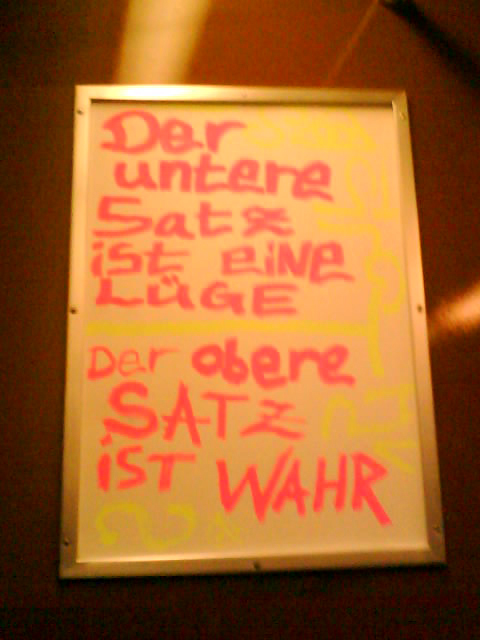
\includegraphics[scale=0.3]{material/13Pragv}

\end{figure}

\end{frame}


%%%%%%%%%%%%%%%%%%%%%%%%%%%%%%%%%%%%%%%
%%%%%%%%%%%%%%%%%%%%%%%%%%%%%%%%%%%%%%%
%
\subsection{Präsupposition}
%
%%%%%%%%%%%%%%%%%%%%%%%%%%%%%%%%%%%%%%%
%\begin{frame
%\frametitle{~}
%	\tableofcontents[currentsection]
%}
%%%%%%%%%%%%%%%%%%%%%%%%%%%%%%%%%%%%%%%

\begin{frame}
\frametitle{Präsupposition}

\begin{itemize}
	\item Implizite Voraussetzung ($\gg$)
	\item Präsuppositionen werden nicht vom Wahrheitsgehalt eines Satzes erfasst
	\item Präsuppositionen müssen erfüllt sein, damit der Satz einen Wahrheitswert haben kann!

\vspace{1ex}

		\ea \label{ex11} Der gegenwärtige König von Frankreich ist kahlköpfig.
		\z
		
		\begin{itemize}
			\item \ref{ex11} ist wahr, wenn es einen kahlköpfigen König von Frankreich gibt.
			\item\ref{ex11} ist falsch, wenn es keinen kahlköpfigen König von Frankreich gibt.
			\item \ref{ex11} kann keinen Wahrheitswert zugeordnet werden, wenn \gqq{es keinen König von Frankreich gibt}.
		\end{itemize}
	
\end{itemize}

\end{frame}



%%%%%%%%%%%%%%%%%%%%%%%%%%%%%%%%%%%%%%%%%%%%%%%%%%%%%%%%%%%%%%%%

\begin{frame}
\frametitle{Präsupposition}

\begin{itemize}
	\item Semantische Präsupposition  (Bedingung für Wahrheit):
	
	\begin{itemize}
		\item p präsupponiert semantisch q, gdw.

		\begin{itemize}
			\item in allen Welten, in denen p wahr ist, auch q wahr ist,
			\item in allen Welten, in denen p falsch ist, q wahr ist.
		\end{itemize}

	\end{itemize}
	
\vspace{1ex}

	\item Pragmatische Präsupposition (Sprachgebrauch):
	
	\begin{itemize}
		\item Ein Sprecher S präsupponiert (pragmatisch) q mit der Äu\ss{}erung von p, wenn er davon ausgeht, dass q gemeinsames Sprecher-Hörer-Wissen ist.
	\end{itemize}
	
\end{itemize}

\end{frame}


%%%%%%%%%%%%%%%%%%%%%%%%%%%%%%%%%%%%%%%%%%%%%%%%%%%%%%%%%%%%%%%%%%%

\begin{frame}
\frametitle{Präsuppositionstests}

\begin{itemize}
	\item Zur Unterscheidung von Präsuppositionen und Assertionen (wahrheitsfunktionaler Gehalt einer Äu\ss{}erung)
	\item[]
	\item \textbf{Negationstest}
	
	\begin{itemize}
		\item Präsupposition bleibt erhalten (vgl. semantische Implikation)		
		
		\ea Maria hat aufgehört zu rauchen.\\ $\gg$ Maria hat geraucht.
		\z
		
		\ea Es ist nicht der Fall, dass Maria aufgehört hat zu rauchen.\\ $\gg$ Maria hat geraucht.
		\z
		
	\end{itemize}	

\end{itemize}	



\end{frame}


%%%%%%%%%%%%%%%%%%%%%%%%%%%%%%%%%%%%%%%

\begin{frame}
\frametitle{Präsuppositionstests}

\begin{itemize}
	\item \textbf{Modalisierungstest}
	
	\begin{itemize}
		\item Präsupposition bleibt erhalten (vgl. semantische Implikation)

		\ea Peters Freundin ist krank.\\ $\gg$ Peter hat eine Freundin.
		\z
		
		\ea Peters Freundin ist wahrscheinlich/ vielleicht krank.\\ $\gg$ Peter hat eine Freundin.
		\z
	
	\end{itemize}
	
\end{itemize}

\end{frame}


%%%%%%%%%%%%%%%%%%%%%%%%%%%%%%%%%%%%%%%%%%%%%%%%%%%%

\begin{frame}
\frametitle{Präsuppositionstest}

\begin{itemize}
	\item \textbf{Frage- und Aufforderungstest}
	
	\begin{itemize}
		\item Präsupposition bleibt erhalten (vgl. semantische Implikation)

		\ea Peter schlägt immer noch seine Frau.\\ $\gg$ Peter hat seine Frau geschlagen.
		\z
		
		\ea Schlägt Peter immer noch seine Frau?\\ $\gg$ Peter hat seine Frau geschlagen.
		\z
		
		\ea Schlag (immer) noch deine Frau!\\ $\gg$ Peter hat seine Frau geschlagen.
		\z
		
		\end{itemize}

\end{itemize}

\end{frame}


%%%%%%%%%%%%%%%%%%%%%%%%%%%%%%%%%%%%%%% 

\begin{frame}
\frametitle{Präsuppositionstests}

\begin{itemize}
\item \textbf{Konditionalisierungstest}

\vspace{5mm}

	\begin{itemize}
		\item Präsupposition bleibt erhalten (vgl. semantische Implikation)
		
		\ea Auch Andrea studiert noch.\\
			$\gg$ Andrea studierte bisher.\\
			$\gg$ Andere studieren auch.
		\z

			\ea Wenn auch Andrea noch studiert, dann bekommt sie kein Bafög mehr. \\
			$\gg$ Andrea studierte bisher.\\
			$\gg$ Andere studieren auch.
		\z

	\end{itemize}
	
\end{itemize}

\end{frame}


%%%%%%%%%%%%%%%%%%%%%%%%%%%%%%%%%%%%%%%%%%%%%%%

\begin{frame}
\frametitle{Präsuppositionstests}

\begin{itemize}
	\item Präsuppositionen werden nicht durch Wahrheitsbedingungen erfasst.
	
	\begin{itemize}
		\item negierbar, erfragbar, modalisierbar
	\end{itemize}
	
	\item Präsupposition muss erfüllt sein, damit der Satz einen Wahrheitswert haben kann!
	
	\ea \label{ex21} Der gegenwärtige König von Frankreich ist kahlköpfig.
	\z
		
		\begin{itemize}
			\item \ref{ex21} ist wahr, wenn es einen König von Frankreich gibt, der kahlköpfig ist.
			\item \ref{ex21} ist falsch, wenn es einen König von Frankreich gibt, der aber nicht kahlköpfig ist.
			\item \ref{ex21} kann keinen Wahrheitswert zugeordnet werden, wenn \gqq{es keinen König von Frankreich gibt}!
		\end{itemize}

\end{itemize}

\end{frame}


%%%%%%%%%%%%%%%%%%%%%%%%%%%%%%%%%%%%%%%%%%%%%%%

\begin{frame}
\frametitle{Präsuppositionsauslöser}

\begin{itemize}
	\item \textbf{Eigennamen}
	
	\ea Kepler starb im Elend. \\ $\gg$ Es gibt ein Individuum namens Kepler.
	\z

	\item \textbf{Definite DPs}
	
	\ea Der König von Frankreich ist kahlköpfig.\\ 
	$\gg$ Es gibt (genau) einen König von Frankreich
	\z
	
	\item \textbf{Verben der Zustandveränderung}

	\ea Es hat aufgehört zu regnen.\\
			$\gg$ Es hat (mal) geregnet.
	\z

\end{itemize}

\end{frame}


%%%%%%%%%%%%%%%%%%%%%%%%%%%%%%%%%%%%%%%%%%%%%%%

\begin{frame}
\frametitle{Präsuppositionsauslöser}

\begin{itemize}
	\item \textbf{Temporalsätze}
	
	\ea Bevor Sie die Klausur geschrieben haben, hatten Sie Ihre Hausaufgaben zurück bekommen.\\
		$\gg$ Sie haben die Klausur geschrieben.
	\z

	\item \textbf{Temporaladverbien}
	
	\ea Peter ist noch krank.\\
		$\gg$ Peter war krank.
	\z
	
	\item \textbf{Faktive Verben}
	
		\ea Sie wissen, dass Sie abgehört werden.\\
		$\gg$ Sie werden abgehört.
		\z
	
\end{itemize}

\end{frame}


%%%%%%%%%%%%%%%%%%%%%%%%%%%%%%%%%%%%%%%%%%%%%%%

\begin{frame}
\frametitle{Präsuppositionsaufhebung}

\begin{itemize}
	\item Aufhebbarkeit durch
	
\vspace{5mm}

	\begin{itemize}
		\item unmittelbaren Kontext:
		
		\ea Maria hat Peter nicht verlassen.\\
			$\gg$ Maria war mit Peter zusammen.
		\z
		
		\item Maria hat Peter nicht verlassen, denn sie waren nie zusammen.
		
\vspace{5mm}

		\item Diskurskontext:
		
		\ea Peter bedauert, den Wagen gekauft zu haben.\\ 
			$\gg$ Peter hat den Wagen gekauft.
		\z
			
		\item Peter wird nicht bedauern (müssen), den Wagen gekauft zu haben. \\(Auch möglich wenn: Peter den Wagen nicht gekauft hat)
				
	\end{itemize}
					
\end{itemize}


\end{frame}


%%%%%%%%%%%%%%%%%%%%%%%%%%%%%%%%%%%%%%%%%%%%%%%
%
\subsection{Implikatur}
%
%%%%%%%%%%%%%%%%%%%%%%%%%%%%%%%%%%%%%%%%%%%%%%%
%\begin{frame
%\frametitle{~}
%	\tableofcontents[currentsection]
%}
%%%%%%%%%%%%%%%%%%%%%%%%%%%%%%%%%%%%%%%%%%%%%%%


\begin{frame}
\frametitle{Implikatur}

\begin{itemize}
	\item Paul Grice (1989): englischer Philosoph
	\item Implikaturen:\\
Bedeutungsaspekte einer Äu\ss{}erung, die nicht explizit erwähnt wurden \ras Nicht durch die Wahrheitsbedingungen eines Satzes erfassbar

	\begin{itemize}
		\item Explizit Gesagtes \ras semantisch beschreibbar
		\item Nicht explizit Gesagtes \ras implikatiert
	\end{itemize}


	\item Implikation \ras implizieren / folgern
	\item Implikatur \ras implikatieren
	\item[]
	\item Konventionelle Implikaturen (umstritten)
	\item Konversationelle Implikaturen
\end{itemize}

\end{frame}


%%%%%%%%%%%%%%%%%%%%%%%%%%%%%%%%%%%%%%%%%%%%%%%

\begin{frame}
\frametitle{Konventionelle Implikatur}

\begin{itemize}
	\item Konventionelle Implikaturen: umstritten
	\item[]
	\item \textbf{Konventionell} \ras mit der (konventionellen) Bedeutung eines Ausdrucks verbunden
	\item[]
	\item Keinen Einfluss auf die Wahrheitsbedingung des Satzes
	
	\begin{itemize}
	\item Konventionelle Implikatur gehört zu einem Ausdruck dazu, bestimmt aber nicht die Bedingungen, unter denen er wahr ist!
	\end{itemize}
	
\end{itemize}

\end{frame}


%%%%%%%%%%%%%%%%%%%%%%%%%%%%%%%%%%%%%%%%%%%%%%%

\begin{frame}
\frametitle{Konventionelle Implikatur}

\begin{itemize}
	\item[]

	\eal 
	\ex Maria ist schwanger aber fährt Fahrrad.
	\ex Maria ist schwanger und fährt Fahrrad.
	\zl
	
	\item \textit{und} vs. \textit{aber}:
		
	\begin{itemize}
		\item Gleiche Wahrheitsbedingungen
		\item \textit{aber} \ras Kontrast zu einer Erwartung
	\end{itemize}

\vspace{5mm}

	\eal 
	\ex Sogar Maria hat die Klausur bestanden.	
	\ex Maria hat die Klausur bestanden.
	\zl

	\item \textit{sogar}:
		
	\begin{itemize}
		\item Überraschung
	\end{itemize}
		
\end{itemize}

\end{frame}


%%%%%%%%%%%%%%%%%%%%%%%%%%%%%%%%%%%%%%%%%%%%%%%

\begin{frame}
\frametitle{Konventionelle Implikatur}

\begin{itemize}
	\item Du bist Professor. vs. Sie sind Professor.
	
	\begin{itemize}
		\item \textit{du} vs. \textit{Sie}:
		
		\begin{itemize}
			\item Gleiche Wahrheitsbedingung
			\item \gqq{Gesellschaftliches Gefälle}
		\end{itemize}
		
	\end{itemize}
	
	\item[]
	\item Nicht aufhebbar \ras ohne sich selbst zu widersprechen
	\item[]
	\item Ablösbar / abtrennbar
	
	\eal
	\ex Sogar Maria ist schwanger.
	\ex Maria ist schwanger.
	\zl
	
	\end{itemize}

\end{frame}


%%%%%%%%%%%%%%%%%%%%%%%%%%%%%%%%%%%%%%%%%%%%%%%

\begin{frame}
\frametitle{Konversationelle Implikatur}

\begin{itemize}
	\item Konventionelle Implikatur \ras konventionell mit einem Ausdruck verbunden
	\item[]
	\item Konversationelle Implikatur (+ $>$ ) \ras
Folgerungen, die nur in bestimmten Äu\ss{}erungssituationen (d.\,h. in Abhängigkeit vom Kontext) entstehen.

\vspace{5mm}

	\begin{itemize}
		\item Kontext: Nach einem Fussballspiel
		
		\ea A: Wie hat dir das Spiel gefallen?\\
B: Also, das Wetter war sehr gut!
		\z

		\item[] + $>$ Das Spiel hat B nicht gefallen.
	\end{itemize}
	
\end{itemize}

\end{frame}


%%%%%%%%%%%%%%%%%%%%%%%%%%%%%%%%%%%%%%%%%%%%%%%

\begin{frame}
\frametitle{Konversationelle Implikatur}

\begin{itemize}
	\item Basis für konversationelle Implikatur \ras Kooperationsprinzip
	\item[]
	\item Sprecher und Hörer befolgen (i.d.R.) Kooperationsprinzip
	\item Kooperationsprinzip steuert die Konversation
	\item[]
	\item \textbf{Kooperationsprinzip}\\
Gestalte deinen Beitrag zur Konversation so, wie es dem Zweck und der Richtung des Gesprächs angemessen ist.

	\begin{itemize}
	\item Maxime der Qualität
	\item Maxime der Quantität
	\item Maxime der Relevanz
	\item Maxime der Modalität
	\end{itemize}
	
\end{itemize}

\end{frame}


%%%%%%%%%%%%%%%%%%%%%%%%%%%%%%%%%%%%%%%%%%%%%%%

\begin{frame}
\frametitle{Konversationelle Implikatur}

\begin{itemize}
	\item \textbf{Maxime der Qualität}\\
Versuche deinen Beitrag so zu machen, dass er wahr ist (sage nichts, was du für falsch hältst oder wofür du keine Anhaltspunkte hast).
	\item[]
	\item \textbf{Maxime der Quantität}\\
Mache deinen Beitrag so informativ wie erforderlich (nicht mehr und nicht weniger Information als nötig).
	\item[]
	\item \textbf{Maxime der Relevanz}\\
Sage nur Relevantes.
	\item[]
	\item \textbf{Maxime der Modalität}\\
Rede klar und unzweideutig, kurz und bündig, geordnet.
\end{itemize}

\end{frame}


%%%%%%%%%%%%%%%%%%%%%%%%%%%%%%%%%%%%%%%%%%%%%%%

\begin{frame}
\frametitle{Konversationelle Implikatur}

\begin{itemize}
	\item Konversationelle Implikaturen
	
\vspace{5mm}
	
	\begin{itemize}
		\item Durch Befolgung von Maximen
		\item[]
		\item Durch scheinbare Verletzung von Maximen
		\item[]
		\item Durch offensichtliche Hinwegsetzung über eine Maxime
	\end{itemize}
	
\end{itemize}

\end{frame}



%%%%%%%%%%%%%%%%%%%%%%%%%%%%%%%%%%%%%%%

\begin{frame}
\frametitle{Konversationelle Implikatur}

\begin{itemize}
	\item[]

	\ea Syntax war heute mal wieder spannend!
	\z

	\item[] + $>$ Syntax war langweilig

	\begin{itemize}
		\item Verletzung der Qualitätsmaxime (Ironie)
	\end{itemize}

	\ea Schönes Wetter heute.
	\z

		\item[] \textbf{Kontext A}: Es regnet.\\
+ $>$ Das Wetter ist scheu\ss{}lich. 

		\begin{itemize}
			\item Verletzung der Qualitätsmaxime (Ironie)
		\end{itemize}
	
		\item[] \textbf{Kontext B}: Peter redet laut über Frau Müller, sieht aber nicht, dass diese hinter ihm steht. In dieser Situation äu\ss{}ert Maria den Satz.\\
+ $>$ Wechsle schnell das Thema! 
		
		\begin{itemize}
			\item (scheinbare) Verletzung der Relevanzmaxime
		\end{itemize}	
		
	\end{itemize}

\end{frame}


%%%%%%%%%%%%%%%%%%%%%%%%%%%%%%%%%%%%%%%

\begin{frame}
\frametitle{Konversationelle Implikatur}

\begin{itemize}
	\item[]

	\ea Einige Mädchen hatten einen Rock.
	\z

	\item[] + $>$ Nicht alle Mädchen hatten einen Rock.
	
	\begin{itemize}
		\item Befolgung der Quantitätsmaxime
	\end{itemize}

\vspace{5mm}

	\item Kontext: Empfehlungsschreiben für einen Kandidaten für einen Lehrstuhl der Philosophie.

	\ea Sehr geehrte Damen und Herren, Herr X spricht ein gutes Deutsch, seine Handschrift ist leserlich und sein Besuch der Übungen war regelmä\ss{}ig. Mit freundlichen Grü\ss{}en \dots
	\z
	
	\item[] + $>$ Herr X eignet sich nicht für diese Position.

	\begin{itemize}
		\item Verletzung der Quantitäts und/ oder Relevanzmaxime
	\end{itemize}
	
\end{itemize}

\end{frame}


%%%%%%%%%%%%%%%%%%%%%%%%%%%%%%%%%%%%%%%

\begin{frame}
\frametitle{Konversationelle Implikatur}

\begin{itemize}
	\item[]
	
	\ea Gehen Sie zur Tür, drücken Sie den Griff im Uhrzeigersinn so weit hinunter wie möglich und ziehen Sie die Tür dann zu sich heran.
	\z

	\item[] + $>$ Verwenden Sie besondere Sorgfalt darauf, die Tür zu öffnen!\\
+ $>$ Ihnen beschreib ich's lieber ganz genau, bevor Sie wieder was falsch machen. (Spott)

	\begin{itemize}
		\item Verletzung der Maxime der Modalität (Fasse dich kurz!)
	\end{itemize}
	
\vspace{1ex}
	
	\ea Karo ging in den Laden und kaufte sich ein Kleid.
	\z

	\item[] + $>$ Karo ging zuerst in den Laden und kaufte dort ein Kleid.

	\begin{itemize}
		\item Befolgung der Modalitätsmaxime
	\end{itemize}
	
\end{itemize}

\end{frame}


%%%%%%%%%%%%%%%%%%%%%%%%%%%%%%%%%%%%%%%

\begin{frame}
\frametitle{Konversationelle Implikatur}

\begin{itemize}
	\item Konversationelle Implikaturen sind aufhebbar (vgl. konventionelle Implikatur)
	
		\ea Einige sind zur Klausur zugelassen. Sogar alle sind zur Klausur zugelassen!
		\z
	
	\item Konversationelle Implikaturen sind nicht durch eine Paraphrase ablösbar (vgl. konventionelle Implikatur)
	
	\ea Peter trifft eine Frau.\\
Peter begegnet einem Menschen weiblichen Geschlechts.
	\z

	\item[] +> Peter trifft sich nicht mit seiner Frau.
	
\end{itemize}

\end{frame}


%%%%%%%%%%%%%%%%%%%%%%%%%%%%%%%%%%%%%%% 

\begin{frame}
\frametitle{Konversationelle Implikatur}

\begin{figure}
\centering

\begin{minipage}[t]{0.45\textwidth}
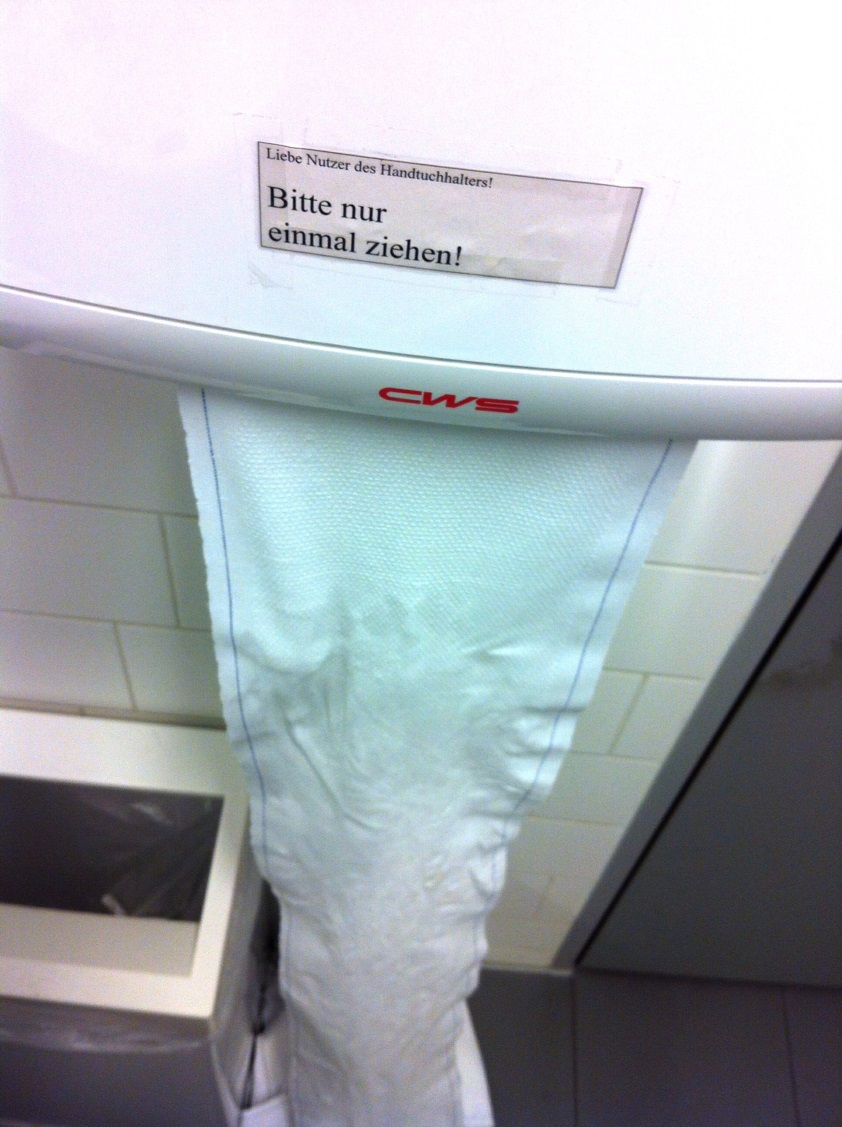
\includegraphics[width=\textwidth]{material/14Prag2}
\end{minipage}
%
\begin{minipage}[t]{0.45\textwidth}
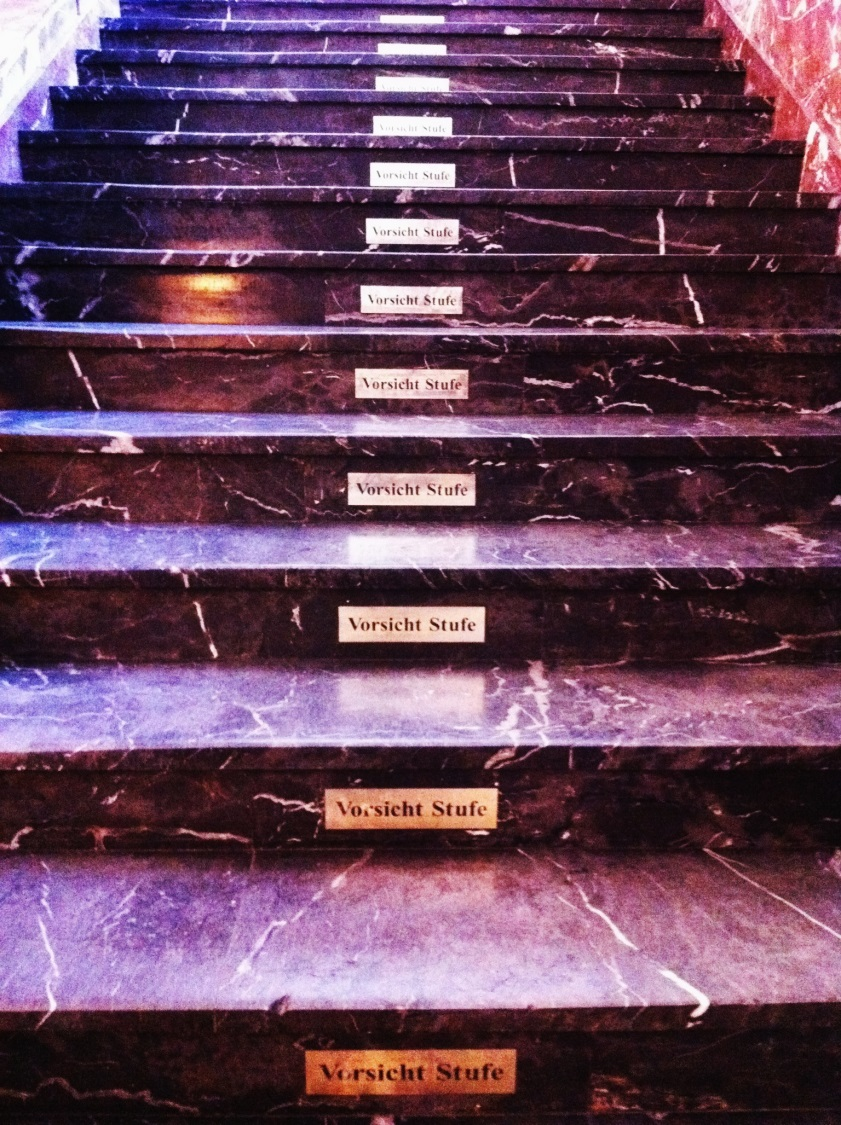
\includegraphics[width=\textwidth]{material/15Prag3}
\end{minipage}

\end{figure}

\end{frame}


%% -*- coding:utf-8 -*-

%%%%%%%%%%%%%%%%%%%%%%%%%%%%%%%%%%%%%%%%%%%%%%%%%%%%%%%%%


\def\insertsectionhead{\refname}
\def\insertsubsectionhead{}

\huberlinjustbarfootline


\ifpdf
\else
\ifxetex
\else
\let\url=\burl
\fi
\fi
\begin{multicols}{2}
{\tiny
%\beamertemplatearticlebibitems

\bibliography{gkbib,bib-abbr,biblio}
\bibliographystyle{unified}
}
\end{multicols}





%% \section{Literatur}
%% \begin{frame}[allowframebreaks]
%% \frametitle{Literatur}
%% 	\footnotesize

%% \bibliographystyle{unified}

%% 	%German
%% %	\bibliographystyle{deChicagoMyP}

%% %	%English
%% %	\bibliographystyle{chicago} 

%% 	\bibliography{gkbib,bib-abbr,biblio}
	
%% \end{frame}


\end{document}


